\section{Theoretical Analysis}
\label{sec:analysis}

For the theoretical simulation, we used the dependent voltage source model of the transistors, with Bf1=178.7 and Bf2=227.3.

The bias circuit, which is constituted by $V_c$, $R_{B1}$ and $R_{B2}$, will determine $V_b$.

To simplify the bias circuit, we can ignore the capacitors and make a Thevenin equivalent. This yields:

\begin{equation}
	R_B=\frac{R_{B1} R_{B2}}{R_{B1}+R_{B2}}
\end{equation}

\begin{equation}
	V_{eq}= \frac{R_{B2}}{R_{B1}+R_{B2}} V_{c}
\end{equation}

To calculate the current that passes through the node 8 we know that $I_E= (1+\beta_f)I_B$

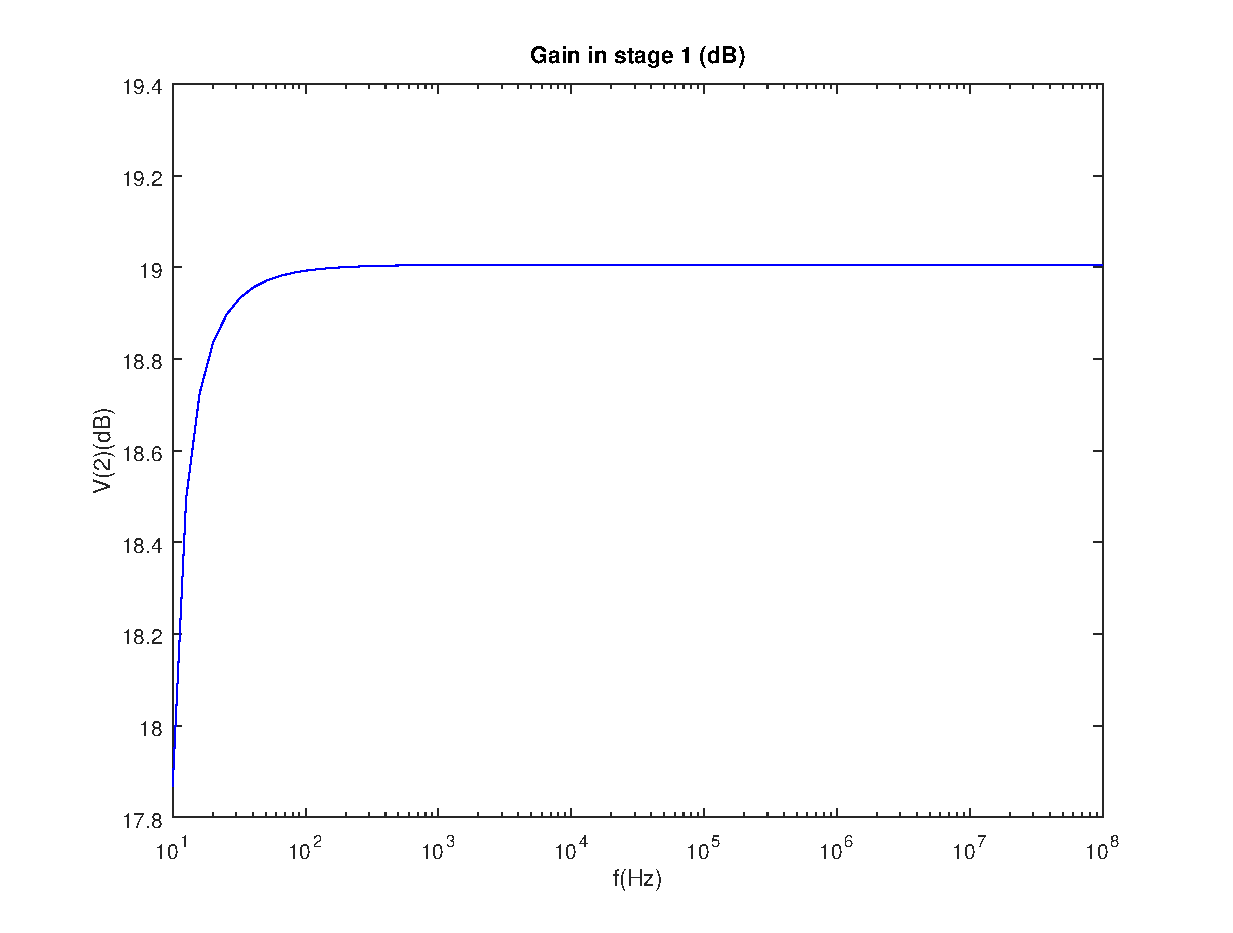
\includegraphics[width=1\linewidth]{vo1.eps}

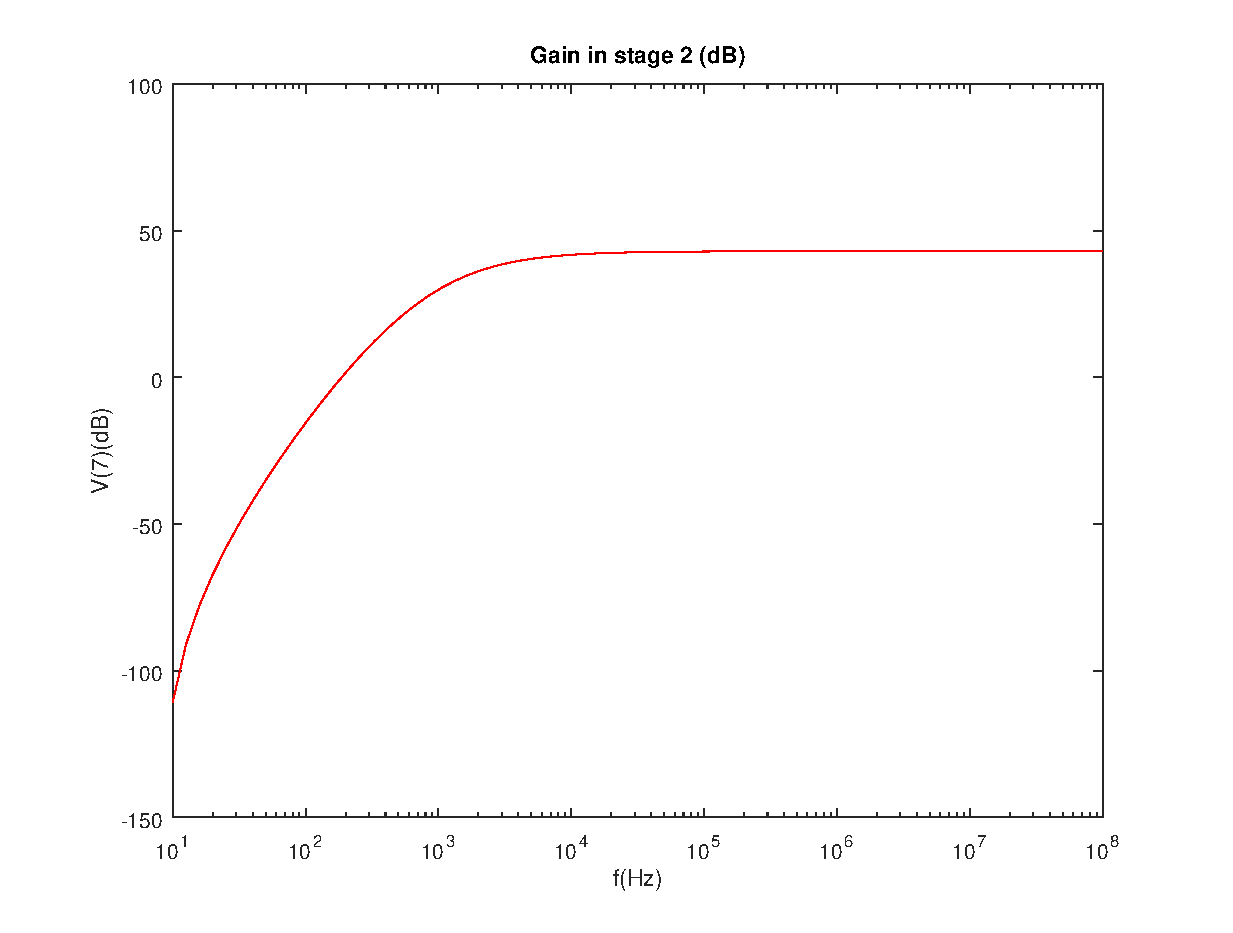
\includegraphics[width=1\linewidth]{vo2.eps}
